\section{Subset Sum \& Knapsack Problem \normalfont{\emoji{money-bag}}}

\subsection{Il Problema}

Il problema delle Subset Sum è formalmente definito come segue:\\

\- abbiamo $n$ oggetti $\{1, \ldots, n\}$, a ognuno viene assegnato un
peso non negativo $w_i$ (per $i = 1, \ldots, n$) e ci viene dato anche un
limite $W$. L'obbiettivo è quello di selezionare un sottoinsieme $S$ degli
oggetti tale che $\sum_{i \in S}w_i \leq W$ e che questa sommatoria abbia valore
più grande possibile.\\

Questo problema è un caso specifico di un problema più generale conosciuto come
il Knapsack Problem, l'unica differenza sta nel valore da massimizzare che per il
Knapsack è un valore $v_i$ e non più il peso.

Si potrebbe pensare di risolvere questi problemi con un algoritmo greedy ma
purtroppo non ne esiste uno in grado di trovare efficientemente la soluzione ottima.
Potremmo pensare di ordinare gli oggetti in base al peso in ordine crescente o
decrescente e prenderli, tuttavia questo approccio fallisce per determinati casi
(come per l'insieme $\{W/2+1, W/2, W/2\}$ ordinato in senso decrescente) e l'unica
opzione sarà quella di provare con la programmazione dinamica \emoji{person-in-manual-wheelchair}.
\newpage

\subsection{\goal}

Possiamo riassumere il goal di questi problemi come segue:\\

\- Abbiamo $n$ oggetti $\{1, \ldots, n\}$, a ognuno viene assegnato un
peso non negativo $w_i$ (per $i = 1, \ldots, n$) e ci viene dato anche un
limite $W$. L'obbiettivo è quello di selezionare un sottoinsieme $S$ degli oggetti
tale che $\sum_{i \in S}w_i \leq W$ e che questa sommatoria abbia valore più
grande possibile.

\subsection{Costi}

\begin{center}
    \begin{tabular}{|c|c|}
        \centering
        \textbf{Funzione}    & \textbf{Costo (tempo)} \\
        \verb|Subset-Sum|    & $O(nW)$                \\
        \verb|Find-Solution| & $O(n)$                 \\
    \end{tabular}
\end{center}

\subsection{Funzionamento}

Come per tutti gli algoritmi dinamici dobbiamo cercare dei sotto-problemi e
possiamo utilizzare la stessa intuizione avuto per il problema dello scheduling
(scelta binaria). Facendo tutti i calcoli di dovere otteniamo la seguente
ricorsione:

\begin{center}
    se $w < w_i$ allora $OPT(i, w) = OPT(i-1,w)$ altrimenti\\
    $OPT(i, w) = max(OPT(i-1, w), w_i + OPT(i-1, w-w_i))$
\end{center}

Nella prima parte analizziamo il caso in cui l'elemento che vogliamo aggiungere va
a superare il peso massimo residuo $w$, dunque viene scartato. Nella seconda parte
andiamo ad analizzare se l'aggiunta o meno del nuovo oggetto va a migliorare
la soluzione di $OPT$ che è definita come:\\

\[
    OPT(i, w) = \max_{S} \sum_{j \in S} w_j
\]
\newpage

Possiamo formalizzare il tutto con il seguente pseudo-codice:

\begin{lstlisting}[language=JavaScript]
    function Subset-Sum(n, W) {
        let M[0 . . . n,0... W]

        //initialize the memoization vector
        for(w in 0 ... W) {
            M[0, W] = 0
        }

        //solve subproblems
        for(i in 1 ... n) {
            for(w in 0 ... W) {
                Use the recurrence to compute M[i, w]
            }
        }

        return M[n, W]
    }
\end{lstlisting}

La particolarità di questo algoritmo è che avremmo 2 insiemi di sotto-problemi
diversi che devono essere risolti per ottenere la soluzione ottima. Questo fatto
si riflette in come viene popolato l'array di memoization dei valori di $OPT$
che verranno salvati in un array bidimensionale.

\begin{figure}[H]
    \centering
    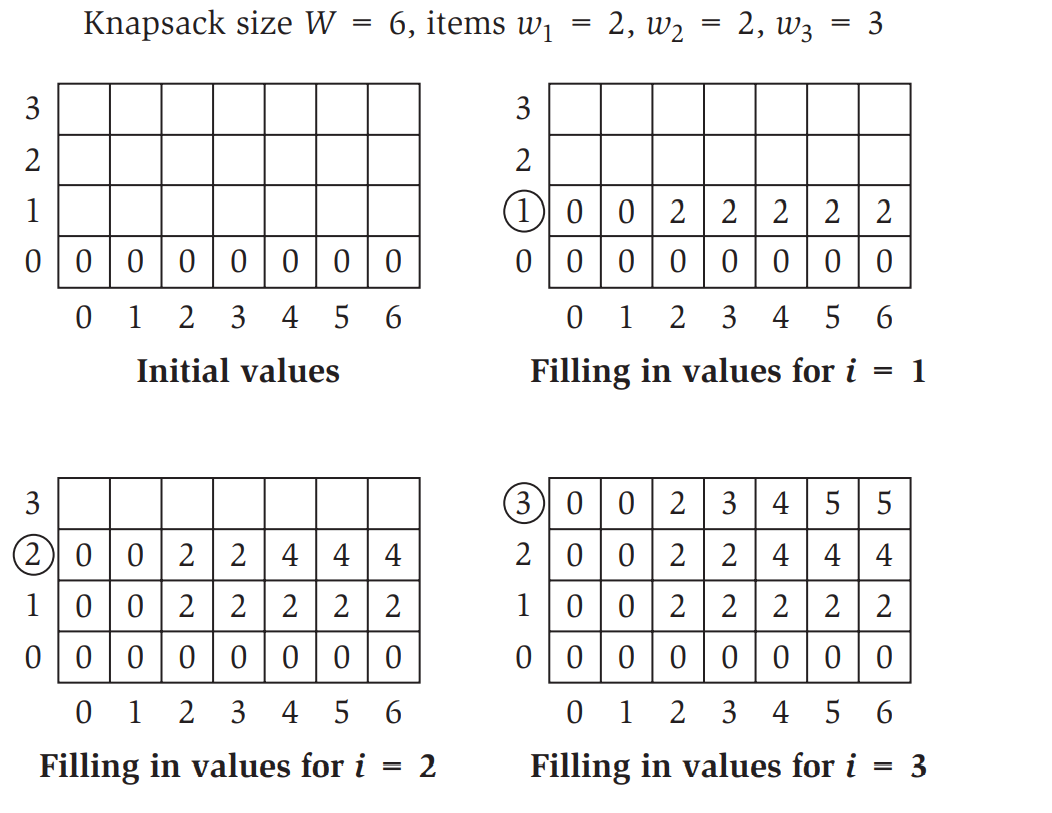
\includegraphics[width=10cm, keepaspectratio]{capitoli/dynamic_programming/imgs/knapsac_table.png}
    \caption{Esempio di come viene popolato l'array $M$ per il problema del Knapsack.}
\end{figure}

\textit{Il costo in tempo di questa implementazione è di $O(nW)$.}\\

A causa di questo costo, l'algoritmo fa parte della famiglia degli
algoritmi \textit{pseudo polinomiali}, ovvero algoritmi il cui costi dipende da
una variabile di input che se piccola, lo mantiene basso e se grande lo fa
esplodere.\\

\textit{Per recuperare gli oggetti dall'array di Memoization la complessità in tempo è di
    $O(n)$.}\\

Questa implementazione funziona anche per il problema più generale del Knapsack,
ci basterà solo cambiare la parte di ricorsione scrivendola come segue:

\begin{center}
    se $w < w_i$ allora $OPT(i, w) = OPT(i-1,w)$ altrimenti
    $OPT(i, w) = max(OPT(i-1, w), v_i + OPT(i-1, w-w_i))$
\end{center}

La complessità temporale è sempre $O(nW)$.